\header{
    \headtitle{Il était une bergère} \label{il-etait-une-bergere}
    %
    
    \insertComment{Variante de "Bergère" de Alain Lotrian (1543).}{}
}

\enluminure{4}{\href{https://www.youtube.com/watch?v=X9kQ5zumZww}{I}}{l était} une bergère
\\Et ron et ron petit patapon,
\\D'humeur assez légère
\\Qui aimait les garçons ron ron,
\\Bien plus que ses moutons.
\dualcol{
Un jour près d'une rivière,
\\Et ron et ron petit patapon,
\\Voyant son ami Pierre,
\\Elle quitta son jupon ron ron,
\\Et son petit pantalon.
\\\\Le garçon, plein de fièvre,
\\Et ron et ron petit patapon,
\\Se pourléchant les lèvres,
\\S'approcha l'air fripon ron ron,
\\Pour tâter son chaton.
\\\\La bergère, peu sage,
\\Et ron et ron petit patapon,
\\Entrouvrit son corsage,
\\En disant au garçon ron ron
\\Embrasse mes tétons.
\\\\Puis elle ouvrit les cuisses,
\\Et ron et ron petit patapon,
\\Afin que le gars puisse
\\Caresser sans façons ron ron
\\Le duvet de son chaton.
\\\\"Donne ta main", dit-elle,
\\Et ron et ron petit patapon
\\"J'aime la bagatelle
\\Caresse-le sinon sinon
\\Tu auras du bâton".
\\\\Il n'y mit pas la patte,
\\Et ron et ron petit patapon
\\Il n'y mit pas la patte,
\\Il y mit le menton cochon,
\\Il y mit le menton.
\\\\Et le long de la rivière,
\\Et ron et ron petit patapon,
\\Retentit cette prière,
\\N'arrête pas c'est bon, très bon,
\\Une minette au chaton,
\\C'est bon,
\\\\Nous recommencerons, 
\\C'est bon, c'est bon!
\begin{center}
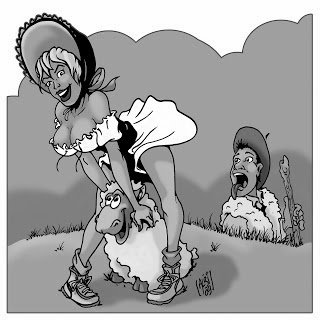
\includegraphics[width=0.45\textwidth]{images/bergere.jpg}
\end{center}
}

\breakpage